\section{Auswertung}
\label{sec:Auswertung}

Im ersten Versuchsteil sollte die Güte des Selektivverstärkers untersucht werden. Dazu
wurde zu verschiedenen Eingangsfrequenzen bei konstanter Amplitude die Ausgangsspannung
vom Filter gemessen. Die dabei aufgenommenen Daten sind in \autoref{tab:filterkurve}
abgedruckt.

\begin{table}
  \centering
  \caption{Messdaten zur Bestimmung der Filterkurve}
  \label{tab:filterkurve}
  \sisetup{table-format=2.1}
  \begin{tabular}{c c}
  \toprule
  $f / \si{kHz}$	& $U / \si{V}$ \\
  \midrule
  18,9&0,08	\\
  20,2&0,09	\\
  22,1&0,12	\\
  23,0&0,14	\\
  27,2&0,205	\\
  29,0&0,26	\\
  31,0&0,44	\\
  32,4&0,5	\\
  33,7&0,42	\\
  33,9&0,51	\\
  34,0&0,5	\\
  34,3&0,55	\\
  35,7&0,66	\\
  36,0&0,64	\\
  36,8&0,54	\\
  37,1&0,49	\\
  39,1&0,28	\\
  41,0&0,19	\\
  42,7&0,16	\\
  42,9&0,33	\\
  46,5&0,14	\\
  52,3&0,09	\\
  \bottomrule
  \end{tabular}
\end{table}

Die Güte ist, wie in \autoref{sec:Theorie} schon erwähnt die relative Breite der Kurve
\[
	Q = \frac{\nu_0}{\nu_+ - \nu_-}.
\]

Für die Berechnung der Güte wird in einer nicht linearen Ausgleichsrechnung eine
Gaußglocke
\begin{equation}
	\label{eqn:gauss-glocke}
	f(\nu) = N * \exp\left(-a \cdot (\nu - \mu)^2\right)
\end{equation}
an die Messdaten gefittet.
\\
Wegen
\begin{equation}
	f(\nu_+) \overset{!}{=} 
	f(\nu_-) \overset{!}{=} 
	\frac{f(\mu)}{\sqrt{2}}
\end{equation}
folgt dann
\begin{equation}
	\label{eqn:nu-plus-minus}
	\nu_\pm = \mu \pm \sqrt{\frac{1}{2a} \ln(2)}
\end{equation}
und 
\begin{equation}
	\label{eqn:Q-Auswertung}
	Q = \frac{\mu}{\sqrt{2/a \ln(2)}}.
\end{equation}

Die nicht lineare Ausgleichsrechnung ergab die Fitparameter
\begin{align}
	\label{eqn:fit-ergebnisse}
	\mu &= (34,8 \pm 0,5) \si{kHz}, \\
	a &= (0,0139 \pm 0,0025) \si{s}, \\
	n &= (0,53 \pm 0,028) \si{V}.
\end{align}

Mit \autoref{eqn:Q-Auswertung} folgt dann unter Verwendung linearer Fehlerfortpflanzung
\begin{equation}
	Q = 3,48 \pm 0,5.
\end{equation}

Die Messdaten und die Ausgleichsfunktion sind in \autoref{fig:filterkurve} dargestellt.

\begin{figure}
	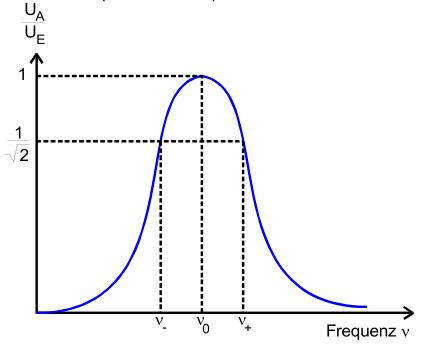
\includegraphics{build/filterkurve.pdf}
	\caption{Plot der Messdaten, der Ausgleichsfunktion sowie der Filterkurve die bei
	$Q=50$ zu erwarten wäre.}
	\label{fig:filterkurve}
\end{figure}

